\documentclass[11pt]{article}
\usepackage[a4paper, margin=2cm]{geometry}
\usepackage[toc, page]{appendix}
\usepackage{graphicx}
\usepackage{hyperref}
\usepackage{enumitem}
\usepackage{subcaption}
\usepackage{amsmath}
\usepackage{multicol}
\usepackage{multirow}
\usepackage{float}
\usepackage{tabularx}
% !TeX spellcheck = en_GB 

\title{Report: Bayesian Networks DAG Testing}
\date{11 November 2018}
\author{Niek Janssen (s4297091)\and Laurens Kuiper (s4467299)\and Ward Theunisse (s4492765)}

\begin{document}
\maketitle
\thispagestyle{empty}
\begin{multicols}{2}
\section{Introduction}
In this report we present the findings of testing and amending the initial model
as proposed in our exposee.  The model was iteratively tested using the
$\chi^2$-test, removing and adding variables/connections at each step.

\section{Initial DAG}
Our initial DAG as shown in \autoref{fig:initial_dag_small} was constructed
with our prior beliefs about the data. A bigger version of this DAG is shown
in the appendix (\autoref{sec:initial_dag} \autoref{fig:initial_dag}). 

\begin{figure}[H]
	\centering
	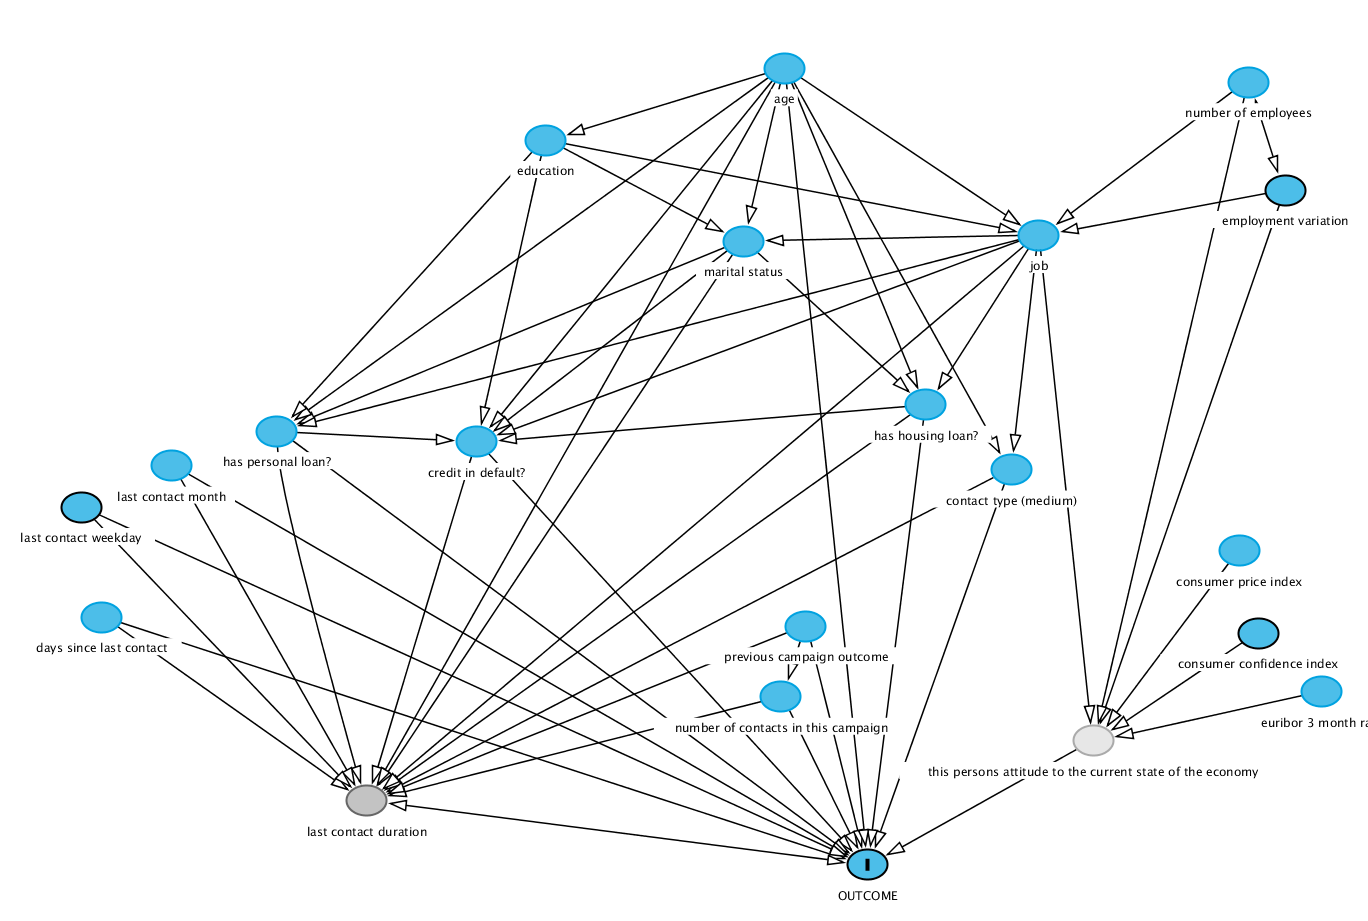
\includegraphics[width=0.4\textwidth]{images/initial_dag}
	\caption{Initial DAG as proposed in expose.}
	\label{fig:initial_dag_small}
\end{figure}

\subsection{Derived Tests}
Conditional independencies were automatically derived using the
\texttt{ImpliedLocalDependencies} function from the \texttt{dagitty} package in
\texttt{R}. The result of this can be found in 
\autoref{sec:initial_conditional_dependencies}. 

\section{Approach}
Tests were performed automatically using the \texttt{localTests} function from
the \texttt{dagitty} package.  However, we are dealing with attributes that can
take on many different values, so we'll need to do some pre processing first.

    \begin{tabular}{ll}
        \textbf{variable} & \textbf{type} \\
        age & Discrete values between 18-85 \\
        nr.employed & continuous values \\
        emp.var.rate & continuous values \\
        cons.price.idx & continuous values \\
        cons.conf.idx & continuous values \\
        euribor3m & continuous values \\
    \end{tabular}

\subsection{Binning}
Because \texttt{dagitty} interprets our data as nominal, it is necessary to bin
our data to allow for meaningful analysis. For each of these attributes, we
inspect the histogram of value frequencies + we apply domain knowledge to obtain
acceptable bins. We explain our binning decisions in the next section.

%Voor elke subsectie nog wat tekst
\subsubsection{Age}
\begin{figure}[H]
	\centering
	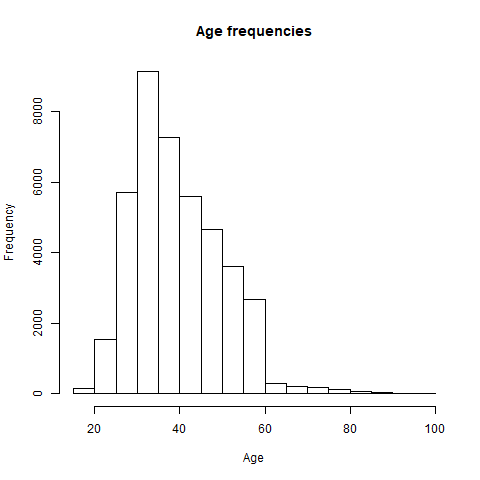
\includegraphics[width=0.4\textwidth]{images/age}
	\caption{Distribution of age.}
	\label{fig:age}
\end{figure}

\subsubsection{Quarterly average of number of employees}
\begin{figure}[H]
	\centering
	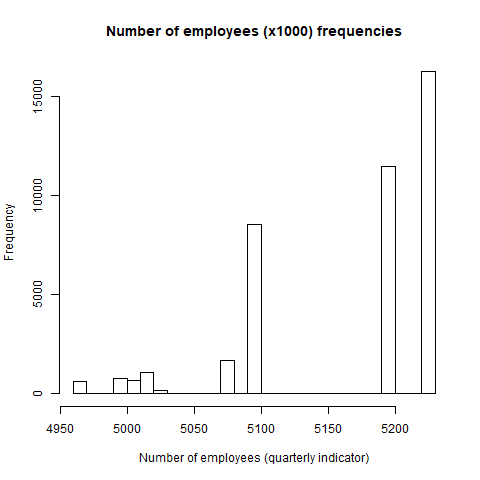
\includegraphics[width=0.4\textwidth]{images/nr_employed}
	\caption{Distribution of number of employees.}
	\label{fig:nr_employed}
\end{figure}

\subsubsection{Quarterly average of number of employees}
\begin{figure}[H]
	\centering
	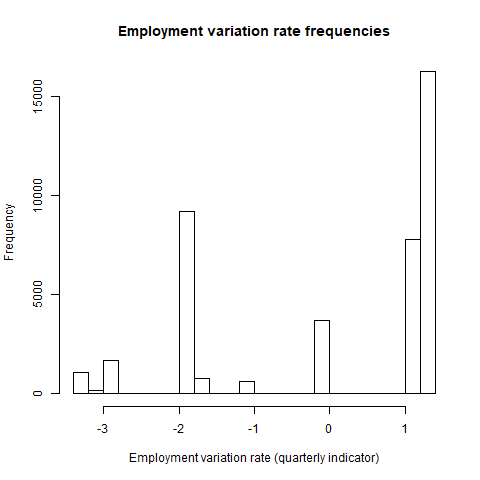
\includegraphics[width=0.4\textwidth]{images/emp_var_rate}
	\caption{Distribution of employment variation rate.}
	\label{fig:emp_var_rate}
\end{figure}

\subsubsection{Consumer price index}
\begin{figure}[H]
	\centering
	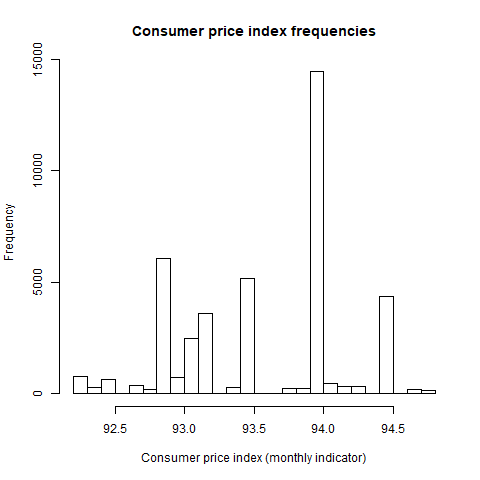
\includegraphics[width=0.4\textwidth]{images/consumer_price_index}
	\caption{Distribution of consumer price index.}
	\label{fig:cons_price_idx}
\end{figure}

\subsubsection{Consumer confidence index}
\begin{figure}[H]
	\centering
	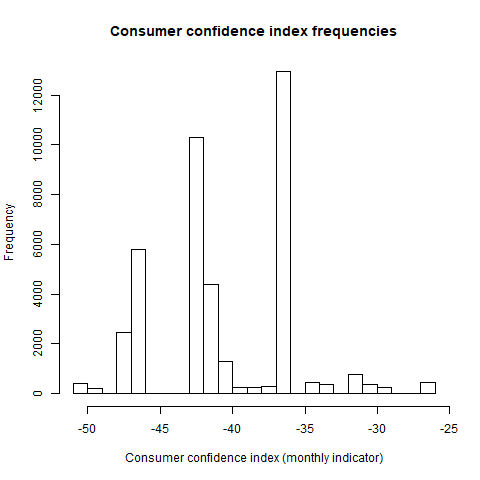
\includegraphics[width=0.4\textwidth]{images/consumer_confidence_index}
	\caption{Distribution of consumer confidence index.}
	\label{fig:cons_conf_idx}
\end{figure}

\subsubsection{Euribor 3 month rate}
\begin{figure}[H]
	\centering
	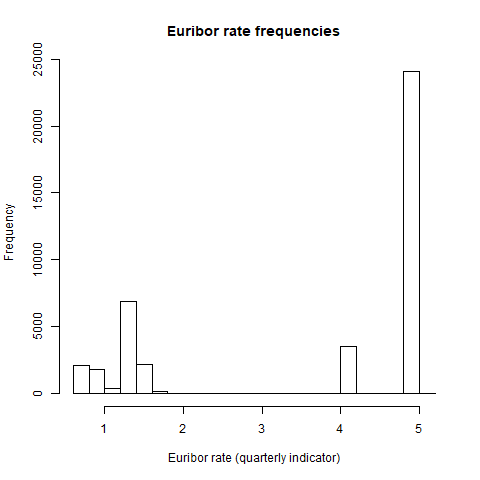
\includegraphics[width=0.4\textwidth]{images/euribor3m}
	\caption{Distribution of three month euribor rate.}
	\label{fig:euribor3m}
\end{figure}

\section{Changes}
We firstly looked at the unconditioned dependencies and added these to our
model when needed. After that, we did the same with the conditioned variables. A changelog
of what we did can be found below. 

\subsection{Contact type}
When we first tested the independencies of our DAG, we found a very strong
dependency between the contact type variable (indicating whether the consumer reached on their cellphone or landline) and the month. After a quick look, this
seemed to be corresponding to the data we have, so we added an arrow from month
to contact type. 

Before we deleted the contact type, though, we found a strong dependency between
default and contact medium, conditioned on age and job. Because the month is
strongly influential on the contact type, we thought it would be most likely
that the month would have a connection with default. We thought it would also be
logical that some months would be more expensive than others, so in these months
people are more likely to have a default. 

We also found a dependency from education to contact. We might be able to
explain this because people with certain jobs need a mobile phone to work
efficiently. 

Later on in the process, we found that the contact type was
continually the same over time, with a single point in time when it switched. The first two years of the data collection was done
via landline, while the last three years all calls were made via a mobile phone.
We finally decided to delete the contact type altogether. 

\subsection{Latent variables}
Education and duration were dependent on each other, conditioned on five other
variables. We added a latent variable called patience. This latent variable
disappeared again when we deleted duration. We removed duration because it highly affects the output target, but it is only known after a call is performed, thus not offering any predictive / actionable information.
The authors of the paper that our data features in state that " this input should only be included for benchmark purposes and should be discarded if the intention is to have a realistic predictive model."

We also found a dependency between loan and housing, conditioned on age, job and
marital status. Another dependency between education and y exists. Because of
this, we add a latent variable "willingness to take a loan". This latent
variable has connections from age, marital status and education, and has
connections to housing, loan and y. All direct connections between these
variables were removed. This latent variable later became wealth, where it has
got connections to marital status and default. 

At first, we thought we could remove patience because the latent variable wealth
would suffice, but this wasn't the case. We could, however, replace it with a
direct connection between education to duration. 

\subsection{More deletions}
Later on, we found that duration is actually dependent on y. This is because,
when people decide that they want a loan (y=true), the call becomes much longer
because of the further administration that has to be done over the phone. This
made us delete the duration altogether. 

Additionally, the vertexes day\_of\_week and campaign got deleted because they
were not meaningfull. 

\subsection{Binning}
We binned the data in following bins:

\medskip
\begin{tabular}{ll}
    \textbf{Variable}           & \textbf{Split on} \\
    Age                         & 18, 25, 30, 45, 60 \\
    Consumer confidence         & 35, 38, 45 \\
    Price index \ 1000          & 92.6, 93.3, 93.6, 94.3 \\
    Empl. var. rate             & -0.5, 0.5, 2.1 \\
    Euribor \ 1000              & 3 \\
    Nr. employed                & 5050, 5150 \\
\end{tabular}

For age, we used our own knowledge, whereas for the economic variables we chose bins that seemed fit the data.

\subsection{Economical variables}
Because we are not economists, we did a little trial and error with the
economical values. All economical variables are updated every three months. The
connections we found are listed in the table below. 

\bigskip
Whether a person has a job depends partly on the global employment and on the
employment variation rate

\medskip
\begin{tabular}{ll}
    \textbf{from} & \textbf{to} \\
    emp.var.rate & job\\
    nr.employed & job 
\end{tabular}

\bigskip
Whether a person can afford a house depends partly on the global economy, so all
four economic variables. This is also true for whether a person needs a loan,
and/or has a default. 

\medskip
\begin{tabular}{ll}
    \textbf{from} & \textbf{to} \\
    emp.var.rate & housing \\
    nr.employed & housing \\ 
    cons.conf.idx & housing \\ 
    cons.price.idx & housing \\ 
    \medskip
    emp.var.rate & loan \\
    nr.employed & loan \\ 
    cons.conf.idx & loan \\ 
    cons.price.idx & loan \\
    \medskip
    emp.var.rate & default \\
    nr.employed & default \\ 
    cons.conf.idx & default \\ 
    cons.price.idx & default \\ 
\end{tabular}

\bigskip
The economical variables also influence eachother. In short: The employment
influences the consumer indexes. This is because the consumer economics do
better when the job market performs better. 

\medskip
\begin{tabular}{ll}
    \textbf{from} & \textbf{to} \\
    emp.var.rate & nr.employed \\
    emp.var.rate & cons.price.idx \\
    emp.var.rate & cons.conf.idx \\
    nr.employed & cons.price.idx \\ 
    nr.employed & cons.conf.idx \\ 
    cons.price.idx & cons.conf.idx \\ 
\end{tabular}


\bigskip
Euribor3m is the average interest of European banks. Banks also change their
interest based on the current economical climate. Because of this, we created
dependencies from euribor3m to all other economical variables. Later on, we
found that a lot of combinations between euribor3m and other economical
variables didn't exist in our data. Combined with the fact that euribor3m only
has two bins, this made the LocalTests function fail. Because the Euribor3m
variable only influences the other economical variables, we could easily delete
it. So we did. 



We found pretty high RMSEA values between marital and economical variables,
conditioned on other economical variables. We think this is a very illogical
dependency, and suspect this is because the strategy of the company has shifted
over time, so they called more people with other marital statuses. 

\section{Revised DAG}
Our revised and final DAG is shown in \autoref{fig:final_dag_small}.  A bigger
version of this DAG is shown in the appendix (\autoref{sec:final_dag}
\autoref{fig:final_dag}). 

\begin{figure}[H]
	\centering
	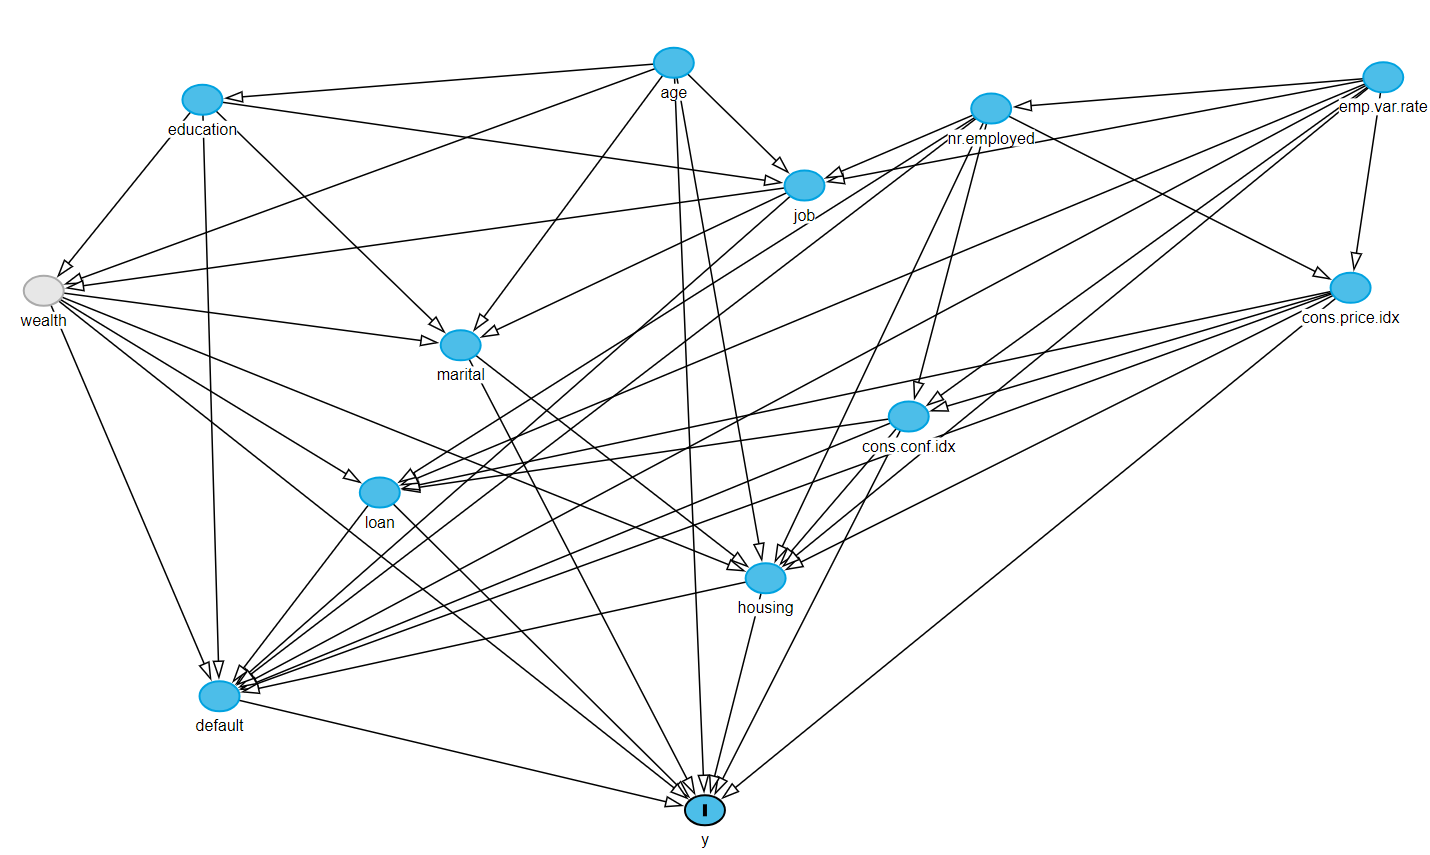
\includegraphics[width=0.4\textwidth]{images/final_dag}
	\caption{Initial DAG as proposed in expose.}
	\label{fig:final_dag_small}
\end{figure}

\subsection{Final RMSEA values}
The final RMSEA values can be found in \ref{sec:final_conditional_dependencies}. 

\newpage
\end{multicols}
\appendix
\section{Initial DAG}
\label{sec:initial_dag}
\begin{figure}[h]
	\centering
	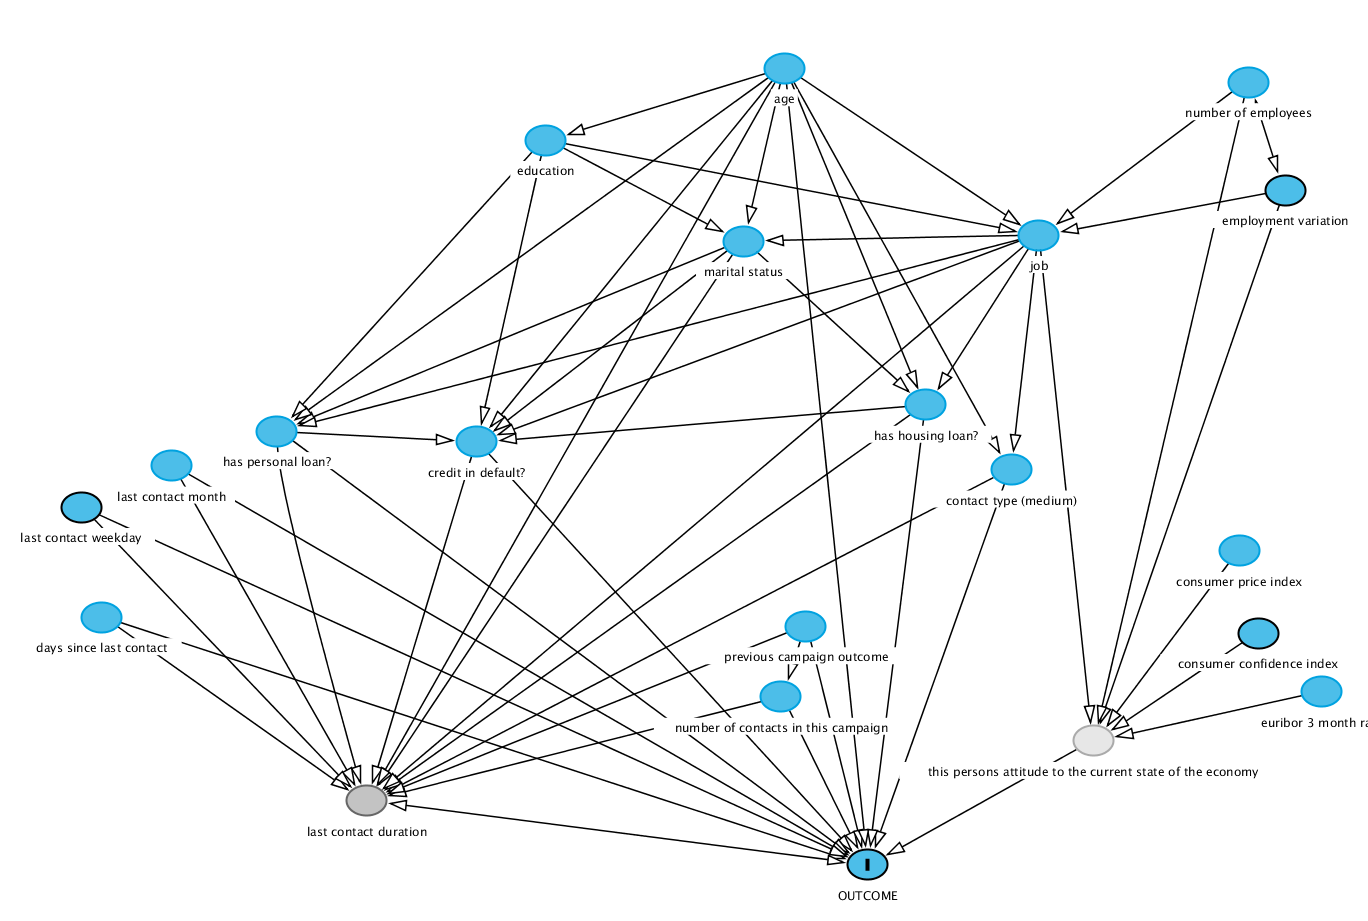
\includegraphics[width=0.8\textwidth]{images/initial_dag}
	\caption{Initial DAG as proposed in exposee.}
	\label{fig:initial_dag}
\end{figure}

\section{Final DAG}
\label{sec:finall_dag}
\begin{figure}[h]
	\centering
	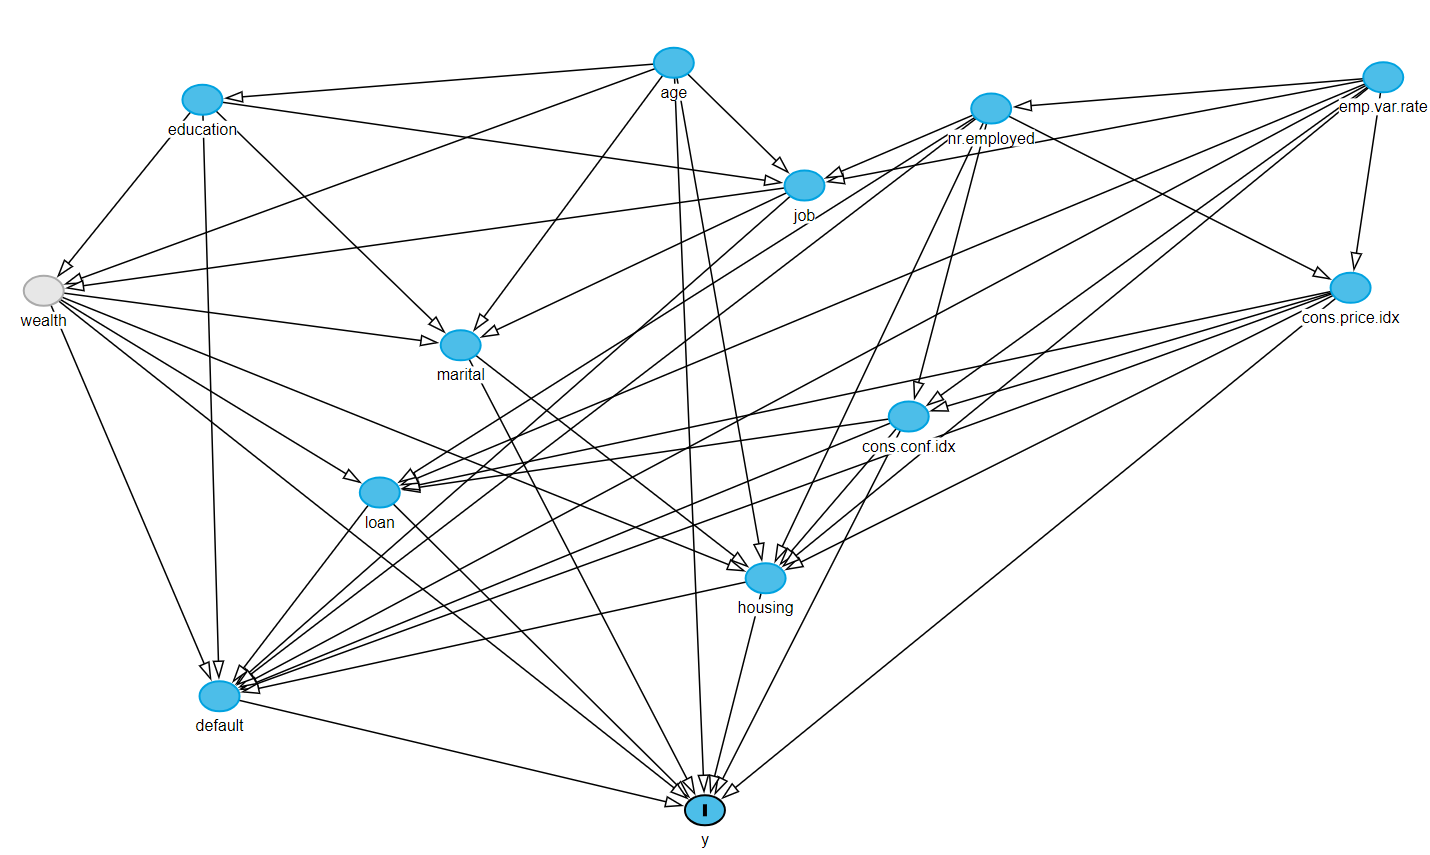
\includegraphics[width=0.8\textwidth]{images/final_dag}
	\caption{Final DAG after model testing.}
	\label{fig:final_dag}
\end{figure}

\newpage
\section{Initial conditional dependencies}
\label{sec:initial_conditional_dependencies}
{\tiny\begin{verbatim}
consumer confidence index _||_ consumer price index
consumer confidence index _||_ contact type (medium)
consumer confidence index _||_ credit in default?
consumer confidence index _||_ days since last contact
consumer confidence index _||_ employment variation
consumer confidence index _||_ euribor 3 month rate
consumer confidence index _||_ has housing loan?
consumer confidence index _||_ has personal loan?
consumer confidence index _||_ last contact duration
consumer confidence index _||_ last contact month
consumer confidence index _||_ last contact weekday
consumer confidence index _||_ marital status
consumer confidence index _||_ number of contacts in this campaign
consumer confidence index _||_ number of employees
consumer confidence index _||_ previous campaign outcome
consumer confidence index _||_ age
consumer confidence index _||_ education
consumer confidence index _||_ job
consumer price index _||_ contact type (medium)
consumer price index _||_ credit in default?
consumer price index _||_ days since last contact
consumer price index _||_ employment variation
consumer price index _||_ euribor 3 month rate
consumer price index _||_ has housing loan?
consumer price index _||_ has personal loan?
consumer price index _||_ last contact duration
consumer price index _||_ last contact month
consumer price index _||_ last contact weekday
consumer price index _||_ marital status
consumer price index _||_ number of contacts in this campaign
consumer price index _||_ number of employees
consumer price index _||_ previous campaign outcome
consumer price index _||_ age
consumer price index _||_ education
consumer price index _||_ job
contact type (medium) _||_ credit in default? | age, job
contact type (medium) _||_ days since last contact
contact type (medium) _||_ employment variation | age, job
contact type (medium) _||_ euribor 3 month rate
contact type (medium) _||_ has housing loan? | age, job
contact type (medium) _||_ has personal loan? | age, job
contact type (medium) _||_ last contact month
contact type (medium) _||_ last contact weekday
contact type (medium) _||_ marital status | age, job
contact type (medium) _||_ number of contacts in this campaign
contact type (medium) _||_ number of employees | age, job
contact type (medium) _||_ previous campaign outcome
contact type (medium) _||_ education | age, job
credit in default? _||_ days since last contact
credit in default? _||_ employment variation | age, education, job
credit in default? _||_ euribor 3 month rate
credit in default? _||_ last contact month
credit in default? _||_ last contact weekday
credit in default? _||_ number of contacts in this campaign
credit in default? _||_ number of employees | age, education, job
credit in default? _||_ previous campaign outcome
days since last contact _||_ employment variation
days since last contact _||_ euribor 3 month rate
days since last contact _||_ has housing loan?
days since last contact _||_ has personal loan?
days since last contact _||_ last contact month
days since last contact _||_ last contact weekday
days since last contact _||_ marital status
days since last contact _||_ number of contacts in this campaign
days since last contact _||_ number of employees
days since last contact _||_ previous campaign outcome
days since last contact _||_ age
days since last contact _||_ education
days since last contact _||_ job
employment variation _||_ euribor 3 month rate
employment variation _||_ has housing loan? | age, job, marital status
employment variation _||_ has housing loan? | age, education, job
employment variation _||_ has personal loan? | age, education, job
employment variation _||_ last contact duration | age, credit in default?, has housing loan?, has personal loan?, job, marital status
employment variation _||_ last contact duration | age, education, job
employment variation _||_ last contact month
employment variation _||_ last contact weekday
employment variation _||_ marital status | age, education, job
employment variation _||_ number of contacts in this campaign
employment variation _||_ previous campaign outcome
employment variation _||_ age
employment variation _||_ education
euribor 3 month rate _||_ has housing loan?
euribor 3 month rate _||_ has personal loan?
euribor 3 month rate _||_ last contact duration
euribor 3 month rate _||_ last contact month
euribor 3 month rate _||_ last contact weekday
euribor 3 month rate _||_ marital status
euribor 3 month rate _||_ number of contacts in this campaign
euribor 3 month rate _||_ number of employees
euribor 3 month rate _||_ previous campaign outcome
euribor 3 month rate _||_ age
euribor 3 month rate _||_ education
euribor 3 month rate _||_ job
has housing loan? _||_ has personal loan? | age, job, marital status
has housing loan? _||_ last contact month
has housing loan? _||_ last contact weekday
has housing loan? _||_ number of contacts in this campaign
has housing loan? _||_ number of employees | age, education, job
has housing loan? _||_ number of employees | age, job, marital status
has housing loan? _||_ previous campaign outcome
has housing loan? _||_ education | age, job, marital status
has personal loan? _||_ last contact month
has personal loan? _||_ last contact weekday
has personal loan? _||_ number of contacts in this campaign
has personal loan? _||_ number of employees | age, education, job
has personal loan? _||_ previous campaign outcome
last contact duration _||_ number of employees | age, education, job
last contact duration _||_ number of employees | age, credit in default?, has housing loan?, has personal loan?, job, marital status
last contact duration _||_ education | age, credit in default?, has housing loan?, has personal loan?, job, marital status
last contact month _||_ last contact weekday
last contact month _||_ marital status
last contact month _||_ number of contacts in this campaign
last contact month _||_ number of employees
last contact month _||_ previous campaign outcome
last contact month _||_ age
last contact month _||_ education
last contact month _||_ job
last contact weekday _||_ marital status
last contact weekday _||_ number of contacts in this campaign
last contact weekday _||_ number of employees
last contact weekday _||_ previous campaign outcome
last contact weekday _||_ age
last contact weekday _||_ education
last contact weekday _||_ job
marital status _||_ number of contacts in this campaign
marital status _||_ number of employees | age, education, job
marital status _||_ previous campaign outcome
marital status _||_ OUTCOME | age, credit in default?, employment variation, has housing loan?, has personal loan?, job, number of employees
marital status _||_ OUTCOME | age, credit in default?, education, has housing loan?, has personal loan?, job
number of contacts in this campaign _||_ number of employees
number of contacts in this campaign _||_ age
number of contacts in this campaign _||_ education
number of contacts in this campaign _||_ job
number of employees _||_ previous campaign outcome
number of employees _||_ age
number of employees _||_ education
previous campaign outcome _||_ age
previous campaign outcome _||_ education
previous campaign outcome _||_ job
OUTCOME _||_ education | age, credit in default?, employment variation, has housing loan?, has personal loan?, job, number of employees
\end{verbatim}}

\section{Final test results}
\label{sec:final_test_results}
{\tiny\begin{verbatim}
                                                             rmsea        x2   df       p.value
age _||_ cons.conf.idx                                  0.08114638 4083.0823   15  0.000000e+00
age _||_ cons.price.idx                                 0.05653150 2652.5172   20  0.000000e+00
age _||_ emp.var.rate                                   0.07828864 3801.5956   15  0.000000e+00
age _||_ nr.employed                                    0.10749941 4769.6201   10  0.000000e+00
cons.conf.idx _||_ education                            0.02926247  761.6302   21 1.223205e-147
cons.conf.idx _||_ job | emp.var.rate, nr.employed      0.02830802  490.7039   66  3.618113e-66
cons.conf.idx _||_ marital | age, education, job        0.12343419 2427.4274 1272  6.928513e-75
cons.conf.idx _||_ marital | emp.var.rate, nr.employed  0.02646795  159.7641   18  9.266606e-25
cons.price.idx _||_ education                           0.04324455 2184.6563   28  0.000000e+00
cons.price.idx _||_ job | emp.var.rate, nr.employed     0.03749213 2051.0141   77  0.000000e+00
cons.price.idx _||_ marital | age, education, job       0.12079377 2896.2705 1557  1.759695e-83
cons.price.idx _||_ marital | emp.var.rate, nr.employed 0.02793123  122.8179   21  2.166818e-16
education _||_ emp.var.rate                             0.02872860  734.8521   21 5.688697e-142
education _||_ nr.employed                              0.03035075  545.1620   14 2.425708e-107
emp.var.rate _||_ marital | age, education, job         0.12642528 2417.9671 1208  3.182673e-83
marital _||_ nr.employed | age, education, job          0.12932179 1626.0104  831  6.335085e-54
\end{verbatim}


\end{document}
